\subsection*{全体概要：この章で学ぶこと}
\addcontentsline{toc}{subsection}{全体概要：この章で学ぶこと}
この章は、ソフトウェアの根本的な形を決め、関係者が共有し、後工程の判断に使うための「アーキテクチャ」を扱う。ここでいうアーキテクチャは、クラス図や構成図そのものではない。図や文書は、アーキテクチャを表すための手段である。アーキテクチャの中心にあるのは、主要な構成要素、それらの関係、設計と進化の原則、品質特性に関するトレードオフ、そして重要な意思決定である。

\noindent 到達目標\quad この章を読み終えると、次のことができるようになる。
\begin{itemize}
  \item 「アーキテクチャ」という語が、分野、活動、成果物の三つの意味で使われることを説明できる。
  \item 利害関係者と関心事を分けて考え、アーキテクチャが誰の何に答えるものかを説明できる。
  \item ビューとビューポイントの違いを説明し、複数の図やモデルを使う理由を説明できる。
  \item アーキテクチャ様式、アーキテクチャパターン、参照アーキテクチャを区別できる。
  \item アーキテクチャ設計を、分析、統合、評価の反復活動として説明できる。
  \item アーキテクチャ評価、レビュー、測度の目的を説明できる。
\end{itemize}

\noindent 学習順序\quad 初学者は、まず「アーキテクチャとは何か」と「利害関係者と関心事」を押さえる。その後、「どう記述するか」「どう設計するか」「どう評価するか」という流れで読むとよい。

\par\smallskip
\begin{center}
\centering
\IfFileExists{assets/generated_figures/ch02/fig-ch02-01.png}{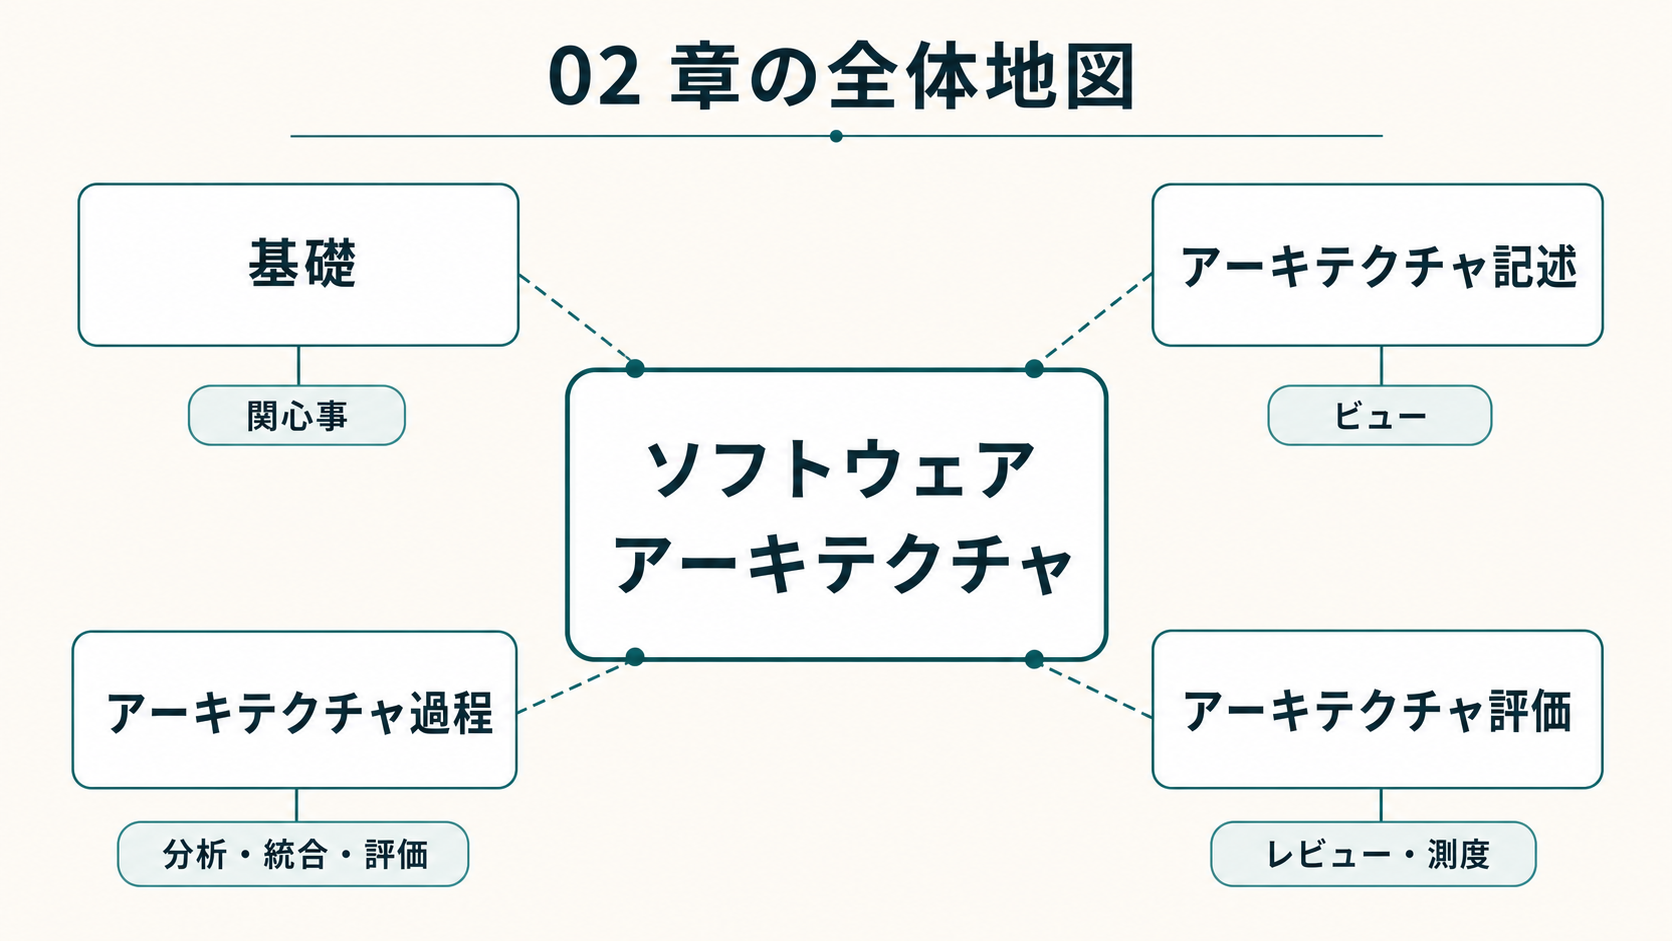
\includegraphics[width=0.96\linewidth]{assets/generated_figures/ch02/fig-ch02-01.png}}{\fbox{\parbox[c][48mm][c]{0.9\linewidth}{\centering 画像生成待ち\\02 章の全体地図}}}
\par\smallskip
\refstepcounter{figure}\label{fig:ch02-01}図 \thefigure: 02 章の全体地図
\end{center}
図 \thefigure は、02 章の全体地図を視覚的に整理したものである。
\par\smallskip

\subsubsection*{最初に必要な用語}
\addcontentsline{toc}{subsubsection}{最初に必要な用語}
\par\smallskip\noindent\refstepcounter{table}\label{tab:ch02-01}表 \thetable: 最初に必要な用語における用語・初学者向けの説明\par\smallskip
表 \thetable は、最初に必要な用語における用語・初学者向けの説明を比較・確認しやすい形で整理したものである。\par\smallskip
\begin{longtable}{P{0.28\linewidth}P{0.64\linewidth}}
\toprule
用語 & 初学者向けの説明 \\
\midrule
ソフトウェア集約システム & ソフトウェアが主要な役割を持つシステムである。ソフトウェアだけでなく、ハードウェア、人、手順、外部サービスも含み得る。 \\
\term{アーキテクチャ}{Architecture} & システムの根本的な概念、構成要素、関係、設計と進化の原則である。単なる図ではなく、重要な判断の集合でもある。 \\
利害関係者 & システムに影響を与える、または影響を受ける人や組織である。顧客、利用者、開発者、運用者、保守担当、監査者などが含まれる。 \\
\term{関心事}{Concern} & 利害関係者が気にする論点である。費用、納期、性能、信頼性、安全性、セキュリティ、使いやすさ、保守しやすさなどである。 \\
品質特性 & システムがどの程度よく振る舞うかを表す性質である。可用性、変更容易性、性能、信頼性、試験容易性などが例である。 \\
\term{アーキテクチャ記述}{Architecture Description} & アーキテクチャを関係者が使えるように、文書、図、表、モデル、意思決定記録などで表した成果物である。 \\
\term{ビュー}{Architecture View} & アーキテクチャの一面を表す図やモデルである。論理ビュー、配置ビュー、開発ビューなどがある。 \\
\term{ビューポイント}{Architecture Viewpoint} & ビューを作り、読み、使うための規約である。記法、表す要素、関心事、想定読者などを定める。 \\
アーキテクチャ上重要な要求 & アーキテクチャに影響する要求である。英語では Architecturally Significant Requirement、略して ASR と呼ぶ。 \\
\term{アーキテクチャ技術的負債}{Architecture Technical Debt} & 今のアーキテクチャ判断が、将来の変更・運用・保守に追加費用を生む状態である。 \\
\bottomrule
\end{longtable}
